\subsection{Temperature distribution on 30 June in Falsterbo}
\label{sec:selected}

Task 3.1 is about the range of temperature for a given day per year. Rebecca's analysis uses the data from Falsterbo weather station to determine the average temperature, standard deviation and probabilities for the day June 30th. The range of years used were from 1880 to 2025. 

\texttt{dailyMeansPerYear} uses a ROOT \texttt{TEntryList} to select the station, month and day and groups the retained observations by year. \testtt{DayHistogram} analyses and plots the relevent data, so that ????


 \texttt{for (Long64_t j = 0; j < elist->GetN(); ++j) {
    tree->GetEntry(elist->GetEntry(j));
 if (year_ < year_from || year_ > year_to) continue;
          sum[year_ - year_from] += measurement_;
          count[year_ - year_from]++;}}

This section of code is taken from day_analysis.cpp. For each entry stored in the elist, GetEntry loads its year and temperature into the variables year_ and measurement_. The continue variable skips the data if the year is outside the range. If the year is inside the range, the temperature is added to the total sum and the count goes up by one. 

\texttt{std::vector<double> values;
for (int k=0; k < nYears; ++k)
        if (count[k] >0) values.push\_back(sum[k]/count[k]);}

The sum can then be divided by the number of counts, which gives the daily mean per year. Therefore, each year with observations contributes one mean temperature, so a year with more readings on the 30th of June contributes the same weight as a year with fewer.


\begin{figure}[htbp]
\centering
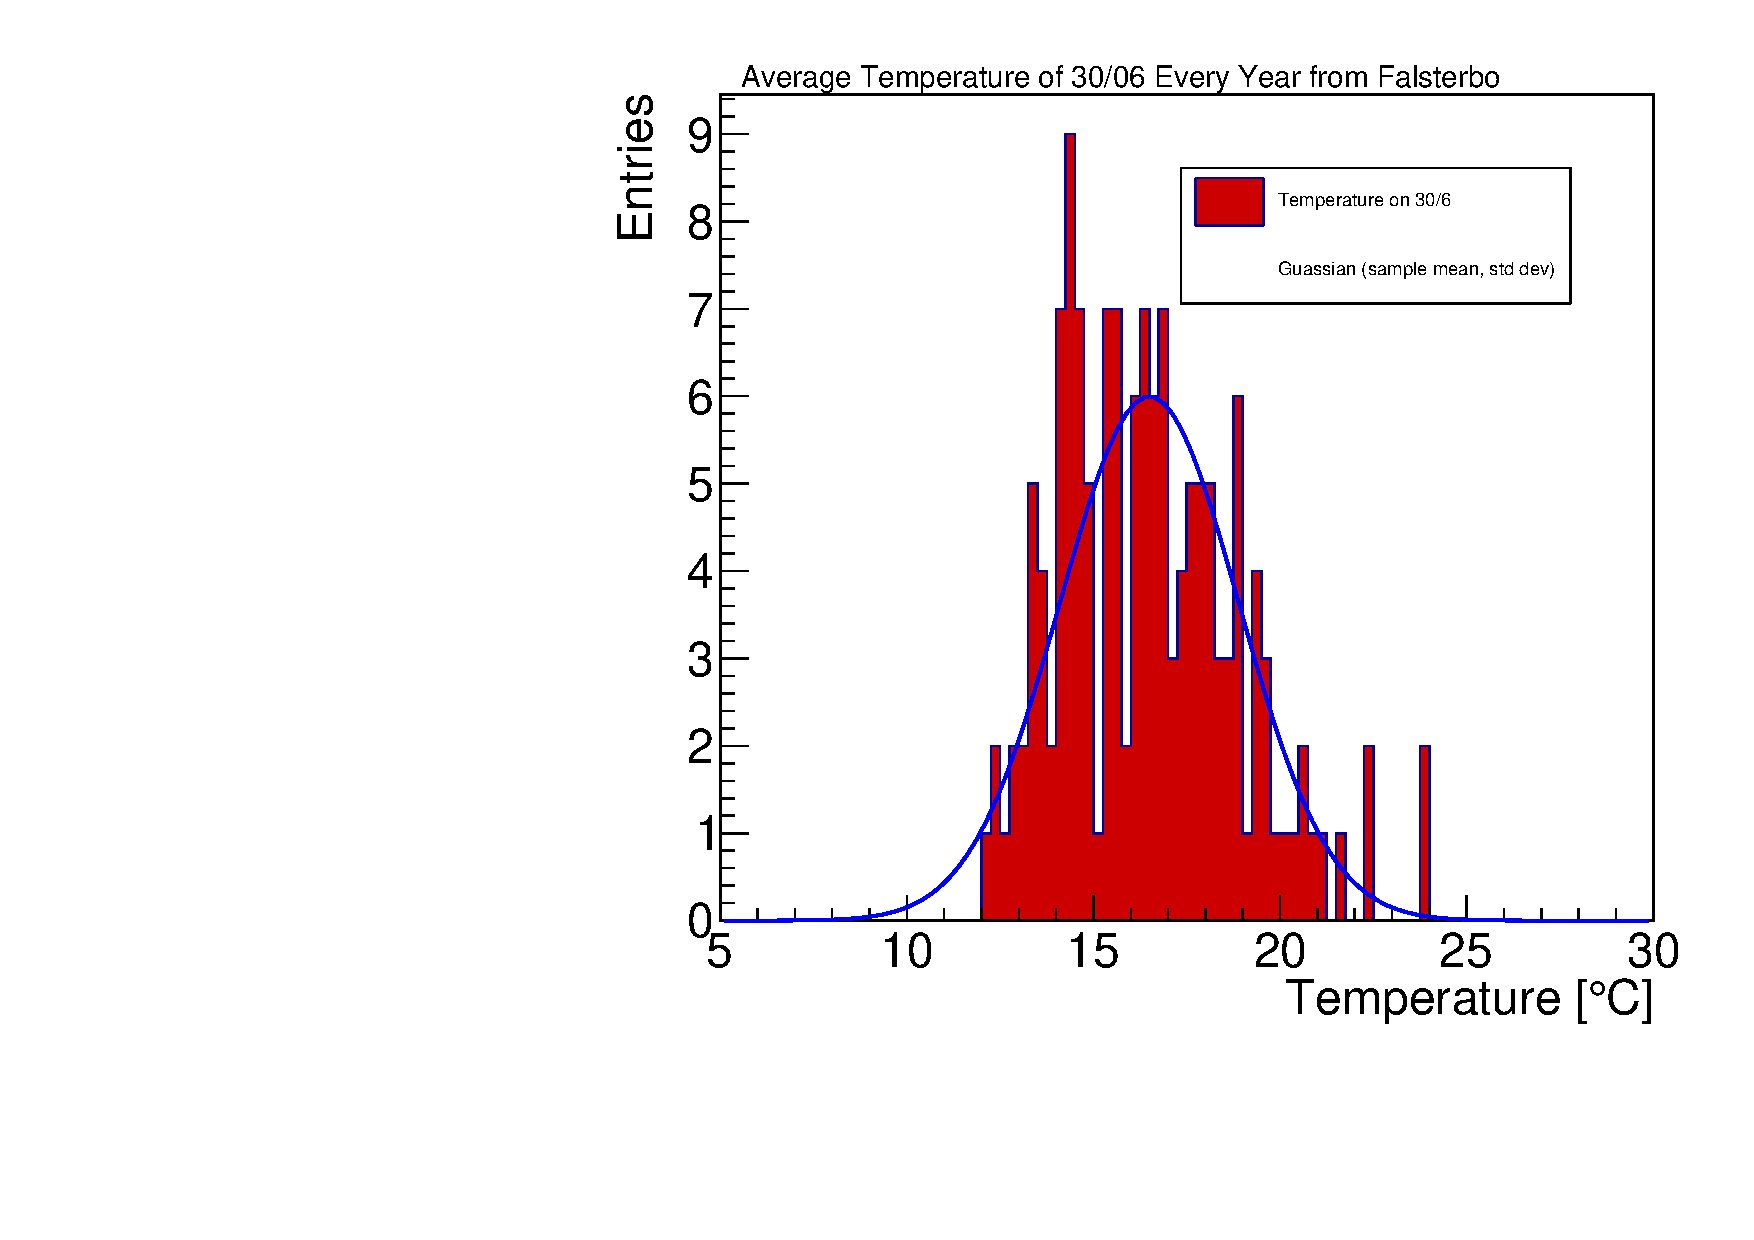
\includegraphics[width=.91\linewidth,height=.40\textheight,keepaspectratio]{Hist_3_with_line.pdf}
\caption{Archived Falsterbo histogram for 30 June with a Gaussian overlay. The entries are daily means from individual years. The curve summarizes the centre and spread of the observed distribution.}
\label{fig:selected}
\end{figure}


The histogram in Figure~\ref{fig:selected} shows that the temperature on 30 June varies appreciably across years, with most entries concentrated near the centre and fewer toward the tails. The histogram shown above uses 100 bins with a temperature range of \(5\deg\) to \(30\degC\). The mean temperature is calculated to be \(16.5\deg\) and the standard deviation to be \(2.4\deg\). A Guassian curve is included in this plots, which uses the mean \(\hat\mu\) and the standard deviation \(\hat\sigma\). The expected curve height scales with the number of observations and the bin width, so it is expressed in the same units as the histogram.

The probability that the data falls into a specific temperature range can be obtained two ways (empirical method $P_1$ and the Guassian method $P_2$). The temperature range was chosen to be \([16,18)\degC\), since this is where most of the data lies. The empirical method takes the years of the data with a daily average that lands in the temperature range and divides by the total number of years. Only 44 years fell into the range. The Gaussian method uses the mean and standard deviation and calculates the probability as the area under the curve between the low and high values.



\begin{align}
  \hat p_{\mathrm{emp}}(d)
    &= \frac{1}{|Y_d|} \sum_{y \in Y_d}
       \mathbf{1}\{a \le \bar T_{y,d} < b\}, \\[4pt]
  \hat p_{\mathrm{G}}(d)
    &= \Phi\!\left(\frac{b-\hat\mu_d}{\hat\sigma_d}\right)
     - \Phi\!\left(\frac{a-\hat\mu_d}{\hat\sigma_d}\right),
\end{align}

The number of standard deviations can be caluclated using $n_\sigma = \frac{|P_1 -P_2|}{SE} = 0.48$, where SE is the standard error of the emprirical probability. This shows that they agree within the uncertainty and that the normal distribution is a reasonable model. The Guassian model also provides the pobability that the temperature with surpass \(T>20\degC\). Both methods pool the available years, so interpreting them as forecasts would require assessing whether the distribution is stable over time.
